%  ========================================================================
%  Copyright (c) 1985 The University of Washington
%
%  Licensed under the Apache License, Version 2.0 (the "License");
%  you may not use this file except in compliance with the License.
%  You may obtain a copy of the License at
%
%      http://www.apache.org/licenses/LICENSE-2.0
%
%  Unless required by applicable law or agreed to in writing, software
%  distributed under the License is distributed on an "AS IS" BASIS,
%  WITHOUT WARRANTIES OR CONDITIONS OF ANY KIND, either express or implied.
%  See the License for the specific language governing permissions and
%  limitations under the License.
%  ========================================================================
%

% Documentation for University of Washington thesis LaTeX document class
% by Jim Fox
% fox@washington.edu
%
%    Revised 2020/02/24, added \caption()[]{} option.  No ToC.
%
%    Revised for version 2015/03/03 of uwthesis.cls
%    Revised, 2016/11/22, for cleanup of sample copyright and title pages
%
%    This document is contained in a single file ONLY because
%    I wanted to be able to distribute it easily.  A real thesis ought
%    to be contained on many files (e.g., one for each chapter, at least).
%
%    To help you identify the files and sections in this large file
%    I use the string '==========' to identify new files.
%
%    To help you ignore the unusual things I do with this sample document
%    I try to use the notation
%       
%    % --- sample stuff only -----
%    special stuff for my document, but you don't need it in your thesis
%    % --- end-of-sample-stuff ---


%    Printed in twoside style now that that's allowed
%
 
\documentclass [11pt, proquest] {uwthesis}[2020/02/24]
 
%
% The following line would print the thesis in a postscript font 

% \usepackage{natbib}
% \def\bibpreamble{\protect\addcontentsline{toc}{chapter}{Bibliography}}

\setcounter{tocdepth}{1}  % Print the chapter and sections to the toc
 

% ==========   Local defs and mods
%

% --- sample stuff only -----
% These format the sample code in this document

\usepackage{alltt}  % 
\newenvironment{demo}
  {\begin{alltt}\leftskip3em
     \def\\{\ttfamily\char`\\}%
     \def\{{\ttfamily\char`\{}%
     \def\}{\ttfamily\char`\}}}
  {\end{alltt}}
 
% metafont font.  If logo not available, use the second form
%
% \font\mffont=logosl10 scaled\magstep1
\let\mffont=\sf
% --- end-of-sample-stuff ---

% Table 5.1
\usepackage{amsmath}
\usepackage{graphicx}
\usepackage{array}

% BibTeX
\usepackage{url}

\begin{document}
 
% ==========   Preliminary pages
%
% ( revised 2012 for electronic submission )
%

\prelimpages
 
%
% ----- copyright and title pages
%
\Title{GhostPeerShare}
\Author{Jeffrey Murray Jr}
\Year{2024}
\Program{Cybersecurity Engineering}

\Chair{Brent Lagesse}{Ph.D}{Computing \& Software Systems}
\Signature{Geethapriya Thamilarasu}
\Signature{Yang Peng}

\copyrightpage

\titlepage  

 
%
% ----- signature and quoteslip are gone
%

%
% ----- abstract
%


\setcounter{page}{-1}
\abstract{%
This sample dissertation is an aid to students who are attempting
to format their theses with \LaTeX, a sophisticated
text formatter widely used by mathematicians and scientists everywhere.
 
\begin{itemize}
\item It describes the use of a specialized
macro package developed specifically for thesis production
at the University.
The macros customize \LaTeX\ for the correct thesis style,
allowing the student to concentrate on the substance of
his or her text.%
\footnote{See Appendix A to obtain the source to this
 thesis and the class file.}
\item It demonstrates the solutions to a variety of
formatting challenges found in thesis production.
\item It serves as a template for a real dissertation.
\end{itemize}
}
 
%
% ----- contents & etc.
%
\tableofcontents
\listoffigures
\listoftables
 
%
% ----- glossary 
%
\chapter*{Glossary}      % starred form omits the `chapter x'
\addcontentsline{toc}{chapter}{Glossary}
\thispagestyle{plain}
%
\begin{glossary}
\item[Fully Homomorphic Encryption (FHE)] A type of encryption that allows computations to be performed on encrypted data without needing to decrypt it, ensuring data privacy throughout the processing.

\item[Cheon-Kim-Kim-Song (CKKS) Scheme] A fully homomorphic encryption scheme that supports approximate arithmetic on real numbers, particularly useful for decimal-based computations.

\item[Microsoft Simple Encrypted Arithmetic Library (SEAL)] An open-source library developed by Microsoft for implementing homomorphic encryption, supporting arithmetic operations on encrypted data.

\item[Kullback-Leibler Divergence (KLD)] A measure of how one probability distribution diverges from a second, reference probability distribution, used in similarity analysis.

\item[Bhattacharyya Coefficient (BC)] A similarity measure that quantifies the amount of overlap between two probability distributions, commonly used in pattern recognition.

\item[Cramer's Distance (CD)] A statistical measure used to quantify dissimilarity between two probability distributions, sensitive to sample size.

\item[Probability Distribution Form (PDF)] A method of representing data where each value indicates the relative frequency of occurrences, used here to represent video frames for similarity analysis.

\item[Cumulative Distribution Form (CDF)] A representation of a probability distribution where each value is the cumulative sum of probabilities up to that point, ensuring the last value is equal to one. Used in similarity analysis for comparing probability distributions.

\item[Flutter] An open-source, cross-platform framework by Google for building natively compiled applications for mobile, web, and desktop from a single codebase.

\item[Dart] A programming language optimized for building fast applications on any platform, used in the development of Flutter apps.

\item[Foreign Function Interface (FFI)] A Dart feature that allows interaction with C libraries, enabling functionalities like encrypted computations within the Dart and Flutter ecosystems.

\item[FFmpeg] A multimedia framework commonly used for video and audio processing, used here for video preprocessing in mobile applications.

\item[OpenCV] An open-source computer vision and machine learning software library that provides tools for image and video processing.

\item[Conan] A dependency management tool used for packaging and managing C++ libraries, facilitating cross-compilation for various platforms.

\item[GitHub Actions] A CI/CD tool that automates tasks such as building, testing, and deploying software, supporting the automation of plugin testing and deployment in this project.

\end{glossary}

 
%
% ----- acknowledgments
%
% \acknowledgments{% \vskip2pc
%   % {\narrower\noindent
%   The author wishes to express sincere appreciation to
%   University of Washington, where he has had the opportunity
%   to work with the \TeX\ formatting system,
%   and to the author of \TeX, Donald Knuth, {\it il miglior fabbro}.
%   % \par}
% }

%
% end of the preliminary pages

%
% ==========      Text pages
%

\textpages
 
% ========== Chapter 1
 
\chapter {Introduction}

This chapter outlines the challenges and limitations of Microsoft's Simple Encrypted Arithmetic Library. Next, we identify beneficiaries and major stakeholders within the Fully Homomorphic Encryption (FHE) domain. Finally, we present a modular interface that grants access to FHE functionality on modern mobile applications.

\section{Problem Statement}
\label{sec:Problem Statement}
The Microsoft Simple Encrypted Arithmetic Library (SEAL) \cite{sealcrypto} requires significant pre-requisite knowledge in C, C++, Kotlin, and Gradle to compile and embed within mobile applications. These prerequisites have limited the accessibility of SEAL, posing a significant obstacle to the adoption within the mobile community.

\section{Stakeholders}
Microsoft was a pioneer in the Fully Homomorphic Encryption research, leading the development of the Simple Encryption Arithmetic Library, SEAL in 2018. SEAL established a foundation for efficient homomorphic encryption, making it accessible for developers and researchers. The open-source community soon contributed to the field with OpenFHE, a flexible, community-driven project that was initially released in 2020. OpenFHE expands upon the capabilities of SEAL, offering a collaborative platform for researchers and developers interested in advancing encryption technology.

Flutter, a versatile and state-of-the-art framework by Google, as of a 2023 study, captures 46\% of the cross-platform framework market [1]. Recognized for its ability to support high-performance, cross-platform applications, Flutter includes a powerful plugin system with a Foreign Function Interface (FFI). This interface enables seamless integration with C libraries, offering null safety, managed memory, and compatibility across major operating systems, including Android, Linux, macOS, iOS, and Windows.

By leveraging Dart, a more portable programming language, developers and security researchers can interact directly with FHE backend libraries. This integration reduces the complexity of working with SEAL or OpenFHE, allowing developers to rapidly build cross-platform applications with homomorphic encryption capabilities. Furthermore, security researchers can extend the application to support additional C/C++ libraries, broadening the scope of FHE implementations and facilitating wider distribution to end-users.

\section{Contributions}
The Pyfhel library (Ibarrondo and Viand, 2021) provides a native Python interface to SEAL cryptosystems, abstracting core SEAL functionalities for easier use. While Pyfhel supports cross-platform compatibility on Windows, Linux, and macOS, it currently lacks support for mobile platforms like Android and iOS. This project adopts a similar approach, creating a modular interface that supports multiple backend libraries and manages them as Dart plugins.

A key contribution of this work is its modular design, which enables the seamless integration and versioning of different backend libraries through Dart plugins. With the use of CMake configurations, each C library can be synchronized and recompiled as new versions become available, simplifying the update process. Automating these compilations reduces maintenance overhead, ensuring that the libraries remain up-to-date with minimal manual intervention.

To assess both the performance and accuracy of the library, we re-implement the Proof of Presence Share methodology. This method calculates similarity scores between videos without exposing their content, providing strong privacy guarantees. We set up cameras from various angles recording simultaneously and compare the videos for similarity, as well as, perform comparisons against other scenes of the same duration. Using a supervised artificial neural network, we classify the distance measures of KLD, Bhattacharya, and Cramer for training and testing so that the model can differentiate between scenes that are similar and those that are distinct. This classification enables us to accurately evaluate the library's effectiveness in identifying matching scenes while maintaining privacy. By analyzing the model’s accuracy across various similarity scores, we gain insight into the precision and reliability of the library in distinguishing matching scenes without revealing the videos’ content.


% ========== Chapter 2
 
\chapter{Background}

This section outlines the technologies and methods used in this research. We start with Flutter, an open-source framework for building cross-platform applications, and highlight its benefits for mobile development. Next, we introduce the Simple Encrypted Arithmetic Library and explain the process of performing computations on encrypted data. Finally, we discuss the distance measures used for privacy-preserving video similarity analysis, focusing on Kullback-Leibler Divergence, Bhattacharyya Coefficient, and Cramer’s Distance. We examine the properties and uses of each metric to show their importance in our work.

\section{Flutter}
Flutter is a modern, open-source software development kit designed to build stylish and efficient applications for mobile, web, and desktop within a single code base. Flutter is built on top of Dart; an object-oriented language with C-style syntax. Dart includes advanced features out of the box such as garbage collection for memory management, synchronous and asynchronous handlers, null safety, and compile-time data type checking. We selected Flutter for its low development cost and a wide variety of plugins.

The plugin at the root of this project's design, the Foreign Function Interface allows the application to invoke functions from pre-compiled C libraries. Each target platform, specifically Windows, Linux, Android, iOS, and macOS requires different methods to compile, however, the fundamental method of invoking C functions and working with native data structures remains the same across platforms. The plugin is limited to transforming primitive data types, e.g. Booleans, Integers, and Characters, restricting the parameters of native C functions to primitive data types. However, a notable workaround to this problem is passing complex objects by memory address, known as pass by reference, for the underlying C library to access the object stored in this stack. 

To facilitate the networking between peer-to-peer Android devices, QuickShare \cite{samsung_quick_2020} was developed by Samsung as a file-sharing utility application for nearby wireless devices. It leverages Bluetooth to discover nearby wireless devices and optionally uses WiFi to transfer large files between two nodes. QuickShare is accessible through a Flutter plugin that enables users to share data using their device's native sharing capabilities. This allows users to easily send content to other apps, such as social media platforms, messaging apps, or email.

Alternatives such as React Native (with JavaScript) or native development languages with Kotlin (Android) and Swift (iOS) involve different compilation methods. React Native is a popular framework for cross-platform development, comparable to Flutter in plugins and community activity, however, lacks the native support of C interoperability and performance. React Native leverages Kotlin and Swift to configure and compile Android and iOS applications, respectively. This approach carries inherent challenges to developing and testing an application, often requiring additional dependencies to handle trivial maintenance. Flutter aims to streamline the process of building cross-platform applications by unifying the codebase, eliminating the need for separate code for each platform. 

\section{Simple Encrypted Arithmetic Library}
\label{sec:Background SEAL}
To perform computations on encrypted data, this project utilizes Simple Encrypted Arithmetic Library (SEAL) \cite{sealcrypto}, an open-source homomorphic encryption library developed by Microsoft. The library supports limited arithmetic including addition, subtraction, and multiplication to be performed directly on encrypted data without needing to decrypt it. We chose SEAL primarily for its maturity, prevalent adoption in research, and use in Proof of Presence Share \cite{Lagesse2021-PopShare}.

SEAL supports three Fully Homomorphic Encryption (FHE) schemes: Brakerski-Fan-Vercauteren (BFV) \cite{fan2012-bfv}, Brakerski-Gentry-Vaikuntanathan (BGV) \cite{brakerski2012-bgv}, and Cheon-Kim-Kim-Song (CKKS) \cite{Cheon2017-CKKS}. BFV and BGV are integer-based FHE schemes that allow for computations on encrypted integers but differ in their ciphertext structure and noise management techniques. BFV encodes the message with the most significant bits of the ciphertext and accumulates more noise growth for each multiplication circuit. When too much noise accumulates, the ciphertext cannot be decrypted. For simpler computations, BFV offers better performance. BGV encodes the message in the least significant bits and manages noise through modulus switching. This difference in noise management makes BGV suitable for deeper computations with many sequential operations. 

CKKS is specifically designed for scenarios where approximate arithmetic is acceptable, and this trade-off allows for more efficient computations on encrypted real numbers. This scheme is efficient in performing computations, by representing real numbers as complex numbers. The encoding allows for efficient arithmetic operations, specifically addition, multiplication, and subtraction. When decoding, the result is transformed into a meaningful representation of the true value, with some degree of error. 

\section{Distance Measures}
\label{sec:Background Distance Measures}
To accurately measure the similarity between the two videos, this project implements the Kullback-Leibler Divergence, Bhattacharyya Coefficient, and Cramer’s Distance. Pop-Share \cite{Lagesse2021-PopShare} established these metrics as an effective indicator for comparing video similarity. Unlike other probability distribution algorithms that involve complex calculations, these three metrics rely primarily on element-wise addition, subtraction, and multiplication of vectors. This simplicity is crucial for their integration with Fully Homomorphic Encryption, as it allows for efficient computation on a list of encrypted floating-point numbers.

Kullback-Leibler Divergence \cite{Kullback1951-bg}, represented as $KLD$ in Equation \ref{eq:kld}, is a state-of-the-art measure of how one probability distribution diverges from a second, expected probability distribution. A limitation of KLD is that it is not symmetric, in that the divergence from distribution P to Q is not necessarily the same as from Q to P, which may complicate its interpretation. The divergence ranges from 0 to positive infinity, where a value closer to 0 indicates high similarity between the distributions.

\begin{equation}
    KLD = \sum_{i} P(i) \log \left( \frac{P(i)}{Q(i)} \right)
    \label{eq:kld}
\end{equation}

Bhattacharyya Coefficient \cite{Bhattacharyya1933-fw}, represented as $BC$ in Equation \ref{eq:bc}, is a measure that quantifies the amount of overlap between two probability distributions. The coefficient ranges from 0 to 1, where a value closer to 1 indicates high similarity between the distributions.

\begin{equation}
    BC(P, Q) = \sum_{x} \sqrt{P(x) Q(x)}
    \label{eq:bc}
\end{equation}

Cramer’s Distance \cite{Cramer1928-sw}, represented as $CD$ in Equation \ref{eq:cd}, is a measure used to quantify the dissimilarity between two probability distributions. It is sensitive to small sample sizes, which can result in inaccuracies. The distance ranges from 0 to 1, where a value closer to 0 indicates high similarity between the distributions.

\begin{equation}
    CD = \sqrt{\sum_{i} (P_{i} - Q_{i})^2}
    \label{eq:cd}
\end{equation}


% ========== Chapter 3
 
\chapter{Related Work}

This section reviews significant advancements in Fully Homomorphic Encryption (FHE) and related methodologies relevant to this project. We begin with an overview of existing FHE libraries. Next, we examine the Proof of Presence Share methodology, an innovative application of FHE to compute video similarity. Finally, we discuss alternative video similarity measures.

\section{Fully Homomorphic Encryption Libraries}

Open-Source Fully Homomorphic Encryption Library, OpenFHE [8], is a state-of-the-art C++ library born from a merger of PALISADE, HElib and HEAAN. OpenFHE supports modern schemes and can be configured to use hardware acceleration.

From existing systems, OpenFHE adapted the modular design of PALISADE [9] with the built-in support of BGV, BFV, CKKS and FHEW schemes. From HElib [10] an efficient homomorphic encryption library primarily focused on BGV and CKKS schemes, pioneered research and early development in this domain. HEAAN [11] was integrated to support arithmetic operations on approximate numbers while other schemes only support integer based arithmetic.

Compared to SEAL, OpenFHE library has an actively growing community with modular integrations of existing systems. The documentation and development guides for OpenFHE are much more modern and comprehensive. However, SEAL is much more established within the research community. Regarding performance, there have not been any peer reviewed publications directly comparing the performance of Microsoft SEAL and OpenFHE.

Python for Homomorphic Encryption Libraries (Pyfhel) [2] offers a robust solution by defining C abstraction methods to translate C++ classes into atomic operations. This abstraction layer modularizes the backend libraries, allowing for support of multiple homomorphic encryption libraries, including SEAL and PALISADE. While this approach is more flexible and supports a drop-in replacement of backend libraries, it contains additional complexity for maintenance of the abstraction layer and version control of backend libraries. This project adopts the methodology used in Pyfhel to implement a similar abstraction in Dart, aiming to provide an efficient and intuitive interface for leveraging homomorphic encryption.

\section{Proof of Presence Share}

Proof of Presence Share (Pop-Share) [11] introduces a novel approach for accurately detecting similar video scenes with strong privacy guarantees, presenting two applications of fully homomorphic encryption deployed within a client-server architecture and a distributed peer-to-peer network. In order to accurately detect similar video scenes, Pop-Share proposed a new application and evaluation of Similarity of Simultaneous Observation (SSO) [12]. 

Developed by Wu and Lagesse, SSO was intended to detect streaming Wi-Fi cameras by comparing the probability distribution between network traffic and recording videos on the network. In addition, SSO contributed a computationally efficient way to transform video frames into probability distribution form to be compared by various statistical measures including JSD, KLD, and DTW. The preprocessing approach of SSO slices the video into one second segments, computes the total number of the bytes for all frames in each segment, and normalizes the byte count array, so that it summates to one. However, JSD and DTW could not be simplified enough to be used in fully homomorphic operations, so Pop-Share leveraged Cramer Distance and Bhattacharyya Coefficient to handle the encrypted similarity score measures.

Pop-Share was developed in 2020, their implementation depended on SEAL 3.3 to handle fully homomorphic operations. Once both videos were preprocessed, the transformation was irreversible, having strong privacy guarantees. In addition, the arrays were encrypted and computed using the plaintext counterpart, resulting in less noise accumulation than when using only ciphertext. In a distributed peer-to-peer application, the initiator shares an encrypted video for the recipient to apply their plaintext array onto the untrustworthy ciphertext. The modified ciphertext was returned to the originator to be decrypted and the summation of the decrypted array represents the corresponding similarity score. This was performed for each similarity score measure. A notable limitation of this approach is that their implementation was tightly coupled with a static version of SEAL, making the results difficult to reproduce.

This method demonstrated that SSO generates a unique, one-way signature of videos that can be used to compare for similarity without access to the content of the video. For this project, the results from Pop-Share serve as a baseline comparator for the modular Flutter re-implementation of the Pop-Share peer to peer application.

An alternative approach focuses on using computer vision to extract privacy-sensitive video objects [13] instead of summarizing video frames per segment. This advanced method is particularly suited for video databases hosted in the cloud, as it requires substantial computational resources for feature extraction and similarity score calculations.

Toward Privacy-Preserving Photo Sharing (P3) [14] presents an innovative photo encoding algorithm that enables the comparison of photos without disclosing the content of the frames. The future work section suggests that this method may also be applicable to videos.

\section{Video Similarity}

As a part of SSO and Pop-Share, a video was represented in probability distribution form, in order to compare two probability distributions, there are many methods to produce a similarity score. In this section, we cover all considerations for generating a similarity score, as well as, acknowledge alternative approaches to comparing videos.

Cramer’s Distance (CD) [15] is a measure used to quantify the dissimilarity between two probability distributions. It is based on the concept of the characteristic function and finds applications in statistical inference and hypothesis testing. One limitation of Cramer’s Distance is its sensitivity to sample size, which can result in inaccuracies, particularly when the sample size is small.

\begin{equation}
    D_C(P, Q) = \sqrt{\sum_{i} (P_{i} - Q_{i})^2}
    \label{eq:cramer}
\end{equation}

Bhattacharyya Coefficient (BC) [16] is a measure that quantifies the amount of overlap between two probability distributions, making it useful in various fields such as pattern recognition and image processing. The coefficient ranges from 0 to 1, where a value closer to 1 indicates higher similarity between the distributions.

\begin{equation}
    BC(P, Q) = \sum_{x} \sqrt{P(x) Q(x)}
    \label{eq:bc_discrete}
\end{equation}

Kullback-Leibler Divergence (KLD) [17] is a widely used measure of how one probability distribution diverges from a second, expected probability distribution. A limitation of KLD is that it is not symmetric, meaning that the divergence from distribution P to Q is not necessarily the same as from Q to P, which may complicate its interpretation.
Jensen-Shannon Divergence (JSD) [18] is a symmetric version of KLD that quantifies the similarity between two probability distributions. It is widely used in information retrieval and clustering. A limitation is that while it provides a measure of similarity, it may not capture finer details of the distributions being compared.

\begin{equation}
    D_{KL}(P || Q) = \sum_{i} P(i) \log \left( \frac{P(i)}{Q(i)} \right)
    \label{eq:kld}
\end{equation}

The Pearson Correlation Coefficient (PCC) [19] measures the linear correlation between two variables, producing a value between -1 and 1. It is a fundamental statistical tool in various fields, including psychology and economics. However, this coefficient assumes a linear relationship and may not capture non-linear associations, which could lead to misleading conclusions in certain contexts.

\begin{equation}
    r = \frac{\sum_{i=1}^{n} (X_i - \bar{X})(Y_i - \bar{Y})}{\sqrt{\sum_{i=1}^{n} (X_i - \bar{X})^2} \sqrt{\sum_{i=1}^{n} (Y_i - \bar{Y})^2}}
    \label{eq:pearson}
\end{equation}


Dynamic Time Warping (DTW) [20] is an algorithm used to measure similarity between two temporal sequences that may vary in speed. It has applications in speech recognition, data mining, and video analysis. One limitation of DTW is its computational complexity, particularly for long sequences, which can make it less suitable for real-time applications. 
Alternatives to SSO are advanced applications on top of existing similarity score algorithms. These novel approaches are typically not restricted to resource-constrained environments.

\begin{equation}
    D(i, j) = \text{dist}(X_i, Y_j) + \min \begin{cases}
        D(i-1, j) \\
        D(i, j-1) \\
        D(i-1, j-1)
    \end{cases}
    \label{eq:dtw_recursive}
\end{equation}

\begin{equation}
    C(i, j) = D(i, j) + \min \begin{cases}
        C(i-1, j) \\
        C(i, j-1) \\
        C(i-1, j-1)
    \end{cases}
    \label{eq:dtw}
\end{equation}


Using content-based algorithms, Shan and Lee [21] presented a series of optimal mapping algorithms to detect similarity between video frames of unequal sizes. In addition, Wu, Zhuang, and Pan [22] present a similar shot graphing algorithm with the intention of identifying similar videos within a large database of videos. An enhancement of Bhattacharyya, was proposed by Loza, Mihaylova, Canagarajah, and Bull [23] to generate a particle filter that would iterate over each sample to predict and resample based on the similarity. Overall, these methods may be adapted to be implemented with fully homomorphic encryption, however they would need to be simplified to use basic arithmetic, and may require many parameters to produce a score.


% ========== Chapter 4
 
\chapter{Design}

This methodology is grounded in a modular design, with each Dart plugin structured to support additional cryptographic libraries and extended functionality. The implementation consists of three core components: two Dart plugins and a Flutter application. The Fully Homomorphic Encryption (FHE) Library Plugin integrates Microsoft SEAL, exposing its FHE capabilities to Dart and Flutter communities. The Distance Measure Plugin provides implementations of Kullback-Leibler Divergence, Cramer Distance, and Bhattacharyya Coefficient, along with their fully homomorphic variants, enabling encrypted distance calculations. Together, these plugins support the Video Similarity Application, a Flutter-based Peer-to-Peer Pop-Share application, which facilitates secure video exchange with strong privacy guarantees.

\section{Fully Homomorphic Encryption Library}
\label{sec:Fully Homomorphic Encryption Library}
This implementation adheres to the core design principle of modularity, remaining agnostic to the underlying C++ library. Instead of directly invoking methods within the plugin, the plugin uses the Bridge and Adapter structural design patterns inspired by the work of Alberto Ibarrondo and Alexander Viand \cite{Ibarrondo2021-Pyfhel}. The Bridge pattern decouples the high-level Dart API from the specific C++ implementation by defining an abstract interface. The Adapter pattern connects the Dart interface to the C++ implementation through a C-based intermediary, translating Dart requests into operations understood by the native library. This approach enables compatibility with multiple Fully Homomorphic Encryption (FHE) backends without modifying the Dart API.

The Fully Homomorphic Encryption Library provides a modular API that integrates Microsoft SEAL with the Flutter ecosystem. It offers a straightforward interface for developers, abstracting low-level complexities while delivering access to advanced encryption functionalities required for secure applications. The topology of this Dart plugin ensures a clear separation of responsibilities to promote maintainability and extensibility. Table \ref{table:class-structure} outlines the distinct roles of each component, including the high-level API, the adapter interface, and the concrete implementation.

\begin{table}[t]
\caption{Class Structure Overview}
\centering
\begin{tabular}{|l|l|p{9cm}|}
\hline
\textbf{File} & \textbf{Class} & \textbf{Description} \\ \hline
seal.dart    & Seal    & Entry-point for the end-user API in Dart \\ \hline
afhe.dart    & Afhe    & Dart adapter connecting to the C interface \\ \hline
fhe.cpp      & N/A     & C interface bridging Dart and C++ \\ \hline
afhe.h       & Afhe    & Pure abstract class defining the FHE contract \\ \hline
aseal.cpp    & Aseal   & Concrete implementation of the Afhe abstraction \\ \hline
\end{tabular}
\label{table:class-structure}
\end{table}


Each file plays a specific role in this architecture. The \textit{seal.dart} file provides the primary entry point for the end-user API, allowing developers to interact with the encryption library in Dart. The \textit{afhe.dart} file acts as the adapter, invoking lower-level C functions. The Afhe class exposes abstracted data types such as Keys, Ciphertext, and Plaintext objects. The \textit{fhe.cpp} file defines the C interface. It exposes the inherited methods from \textit{afhe.h} and references the memory address of the underlying C++ object. Depending on the reference, the corresponding concrete implementation will be invoked. For example, \textit{aseal.cpp} manages Microsoft SEAL objects.

The Foreign Function Interface (FFI) is this plugin's core dependency; It enables Dart to interact with the pre-compiled C binary. For each target platform, the dynamically linked library must be accessible on the local file system. This plugin exposes methods to cast native C data types into Dart objects and vice versa. Our implementation creates Dart objects that mirror their corresponding underlying C++ class. For example, in Microsoft SEAL, a Ciphertext can be saved or loaded. We expose \textit{save\_ciphertext} and \textit{load\_ciphertext} in the C interface. In Dart, we create a Ciphertext class that contains both \textit{save} and \textit{load}, referencing the memory address of the underlying abstract Ciphertext object. This implementation pattern is consistent and transparent for security researchers familiar with the underlying C++ API. For new developers, our implementation mirrors the structure of Microsoft SEAL, providing a clear and familiar interface.

In order to prevent breaking changes, unit tests ensure that the functional behavior of the library remains consistent and reliable throughout the development and release. Unit tests serve as a safety net. They ensure that existing features function as expected when new changes occur. This process reduces the risks of regressions. For SEAL, the authors developed a set of examples that walk the user through their APIs. As a part of the unit tests, we re-implemented these examples with our interface to increase our confidence that our implementation did not introduce any new or unexpected behaviors. For automation, GitHub Actions compiles and executes unit tests using GoogleTest \cite{GoogleTest} with CMake. In total, There are 78 unit tests: 35 in C and 43 in Dart.

In order to distribute this plugin to Linux and multiple Android flavors, GitHub Actions employs Conan \cite{Conan}. Conan automates the management of dependencies and packaging, specifically addressing the versioning of Microsoft SEAL and other backend libraries. For Linux, Conan streamlines the building and packaging process by automatically resolving dependencies tailored to various distributions (e.g., Ubuntu, Fedora, and CentOS) while ensuring compatibility with different versions of Microsoft SEAL and system architectures (e.g., x86, ARM). Similarly, Conan simplifies cross-compilation for Android by allowing developers to specify configurations for various architectures and API levels, ensuring that the plugin can be compiled for the supported CPU architectures x86\_64, ARMv8, and ARMv7. The compiled binaries are all hosted on all platforms and are available for download for each release of the Dart plugin. When developers add the plugin to their dependencies, the binaries are pulled down from GitHub and stored within their local, versioned dependency cache. This automated approach enhances the consistency and reliability of the plugin across different environments, facilitating smoother deployment and easier updates for users.
\section{Distance Measure Plugin}

This Dart plugin calculates three distance measures: Kullback-Leibler Divergence, Cramer Distance, and Bhattacharyya Coefficient, as well as their Fully Homomorphic Encryption (FHE) counterpart. To manage the complexity of these computations, the plugin only supports operations on lists of plaintext doubles, which are then encrypted for processing. In this section, we explain the fully homomorphic computations for each algorithm, along with details on testing and distribution.

%TODO%
Fully homomorphic encryption (FHE) enables computations on encrypted data, ensuring that data privacy is maintained throughout the process. Each algorithm’s encrypted score remains interpretable because it retains the mathematical relationships needed for distance calculation without exposing the underlying plaintext values. For more information on the equations of the plaintext scores, refer to Section 2.3. However, a major limitation in FHE schemes is their inability to directly support division due to the mathematical structures in FHE, which operate within polynomial or modular arithmetic. Workarounds, such as using multiplicative inverses, do exist, though they add complexity and are unreliable.

To accommodate the limitations of FHE, we cannot directly encrypt the input array of doubles for score computation. Instead, we adjust certain parameters tailored to each algorithm’s requirements before encryption. The encrypted parameters and any associated data are stored as binary files, with each algorithm (e.g., $kld\_logX$) using 60 binary files, each representing one second of a one-minute video. This structure is particularly helpful for cases where video lengths differ, as it simplifies the trimming process. The binary files are then archived into an .enc file format, which is unique to our application and contains both the encrypted data and a metadata JSON file with relevant video details (e.g., timestamp, length, frames per second). The archive averages around 2 MB on Linux for 1 minute of video.

To compute the encrypted Kullback-Leibler Divergence using FHE, noted as $KLD_{enc}$ in Equation \ref{eq:fhe_kld_enc}, the ciphertext modification requires three parameters: $X$, $logX$, and $Y$, where $X$ and $logX$ are encrypted arrays, and $Y$ is plaintext. The modified ciphertext is obtained by multiplying each encrypted double in $X$ by the difference between $logX$ and $logY$. This yields an encrypted list of doubles, which, when decrypted and summed, results in the divergence of $Y$ from $X$, shown in Equation \ref{eq:fhe_kld_decrypt}.

\begin{equation}
        KLD_{enc} = ( \log(X)_{enc}^i - \log(Y_{plain}^i) ) \cdot X_{enc}^i
    \label{eq:fhe_kld_enc}
\end{equation}

\begin{equation}
        KLD_{plain} = \sum_{i=1}^{n} D_K(KLD_{enc})
    \label{eq:fhe_kld_decrypt}
\end{equation}

For the Bhattacharyya Coefficient, indicated as $BC_{enc}$ in Equation \ref{eq:fhe_bc_enc}, the square root of $X$ is taken before encryption. This calculation involves two arrays, $sqrtX$ and $Y$, both floating-point arrays. We multiply each encrypted double in $sqrtX$ by the square root of $Y$, yielding an encrypted list. Decrypting and summing this list gives the measure of overlap between the two probability distributions, shown in Equation \ref{eq:fhe_bc_decrypt}.

\begin{equation}
    BC_{enc} = (\sqrt{X})_{enc}^i \cdot \sqrt{Y_{plain}^i}
    \label{eq:fhe_bc_enc}
\end{equation}

\begin{equation}
    BC_{plain} = \sum_{i=1}^{n} D_K(CD_{enc})
    \label{eq:fhe_bc_decrypt}
    \title{Foo}
\end{equation}

To calculate the Cramer Distance, or $CD_enc$ in Equation \ref{eq:fhe_cd_enc}, the cumulative distribution of $X$ is computed iteratively so that the last element sums to one. This requires two arrays, $X$ and $Y$, of floating-point numbers. The computation squares the difference between corresponding elements in $X$ and $Y$, resulting in an encrypted list of values, which, when decrypted, summed, and square-rooted, provides the distance between the distributions, shown in Equation \ref{eq:fhe_cd_decrypt}.

\begin{equation}
    CD_{enc} = (X_{i} - Y_{i})^2
    \label{eq:fhe_cd_enc}
\end{equation}

\begin{equation}
    CD_{plain} = \sqrt{\sum_{i=1}^{n} D_K(CD_{enc})}
    \label{eq:fhe_cd_decrypt}
\end{equation}

The plugin undergoes automated testing via GitHub Actions, which validates scores generated from identical input data to within a 7-decimal-point precision (as shown in Table \ref{table:mean-error}, which details the noise introduced by FHE). Testing covers both the symmetric and asymmetric behavior of each algorithm. A core design goal of this library is modularity, allowing for the future integration of additional distance measures using FHE. This work introduces the FHEL Dart plugin, creating a foundational Dart plugin for distance measurements that supports fully homomorphic encryption.

\section{Video Similarity Application}
\label{sec: Video Similarity Application}
To perform computations on encrypted floating-point numbers, we utilize the CKKS scheme [11] with a polynomial modulus degree of 4096. CKKS is a homomorphic encryption scheme to perform computations of approximate arithmetic on real numbers. This scheme offers out-of-the-box support for decimal value computations compared to other schemes like BFV and BGV, which primarily focus on integer arithmetic. The choice of 4096 as the polynomial modulus degree balances the need for strong security and accuracy with practical computational performance. A larger degree enhances security and allows for more operations before result degradation, with the trade-off of increasing computation time and ciphertext size.

In order to detect similarities between the two videos, we represent each video as a probability distribution of byte size changes between one-second segments, shown in Figure \ref{fig:preprocess-data-flow}. To transform raw video into comparable probability distributions, we count the number of bytes in each frame, calculate the sum of frame lengths in each segment, and then normalize the array of segments between zero and one, known as a Probability Distribution Form (PDF), ensuring that the distributions for both videos have the same scale and can be directly compared. This re-implementation of Proof of Presence Share \cite{Lagesse2021-PopShare} provides strong privacy guarantees, as if the encryption is broken, the raw byte data cannot be reconstructed from the normalized byte array due to the loss of information during the aggregation and normalization process. Alternative approaches include a motion estimation approach with the Lucas-Kanade method \cite{Lucas1981-uy} supported by OpenCV, which could provide more detailed information about video content. However, for this study, it is crucial to compare our approach to the established baseline metrics, and new methods would hinder this comparison.

\begin{figure}[t]
    \centering
    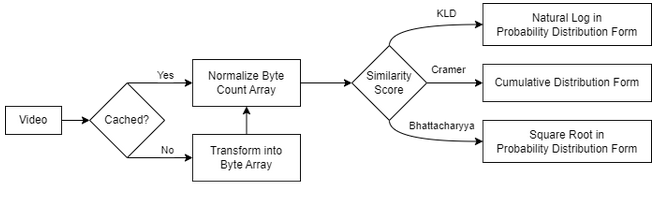
\includegraphics[width=\textwidth]{4 Design/4.3 Preprocess Data Flow.png}
    \caption{Pre-process Data Flow}
    \label{fig:preprocess-data-flow}
\end{figure}

To compute multiple similarity scores using homomorphic encryption, separate byte arrays are encrypted for each score. The recipient can perform computations with plaintext decimal values against the corresponding encrypted element in the array. This approach leverages the unique ability of fully homomorphic encryption and was borrowed from Pop-Share, as this approach is much faster than comparing ciphertext against ciphertext. 

For Kullback-Leibler Divergence, we share the PDF and its natural log. For each encrypted double in the PDF, we subtract the natural log of the plaintext element and multiply the difference. The product remains encrypted and is returned to the originator, where it can be decrypted. The summation is the similarity score.

For Bhattacharyya Coefficient, we share the square root of the PDF. For each encrypted double, we multiply the ciphertext by the square root of the plaintext element. The product remains encrypted and is returned to the originator, where it can be decrypted. The summation is the similarity score.

For Cramer Distance, we share the Cumulative Distribution Form (CDF) from PDF. The CDF is the cumulative sum of all of the elements in the PDF, such that the last value of CDF is equal to 1. For each encrypted double, we square the difference of the plaintext element. The product remains encrypted and returned to the originator, where it can be decrypted, and the square root of the summation is the similarity score.

In order to share the encrypted byte-count arrays, GhostPeerShare packages all ciphertext objects into an archive. The encrypted parameters and any associated data are stored as binary files, with each algorithm (e.g., $kld\_logX$) using 60 binary files, each representing one second of a one-minute video. This structure is particularly helpful for cases where video lengths differ, as it simplifies the trimming process. The binary files are then archived into an \textit{.enc} file format, which is unique to our application and contains both the encrypted data and a metadata JSON file with relevant video details (e.g., timestamp, length, frames per second). The archive averages around 40 MB on Linux for 1 minute of video.

\begin{figure}[t]
    \centering
    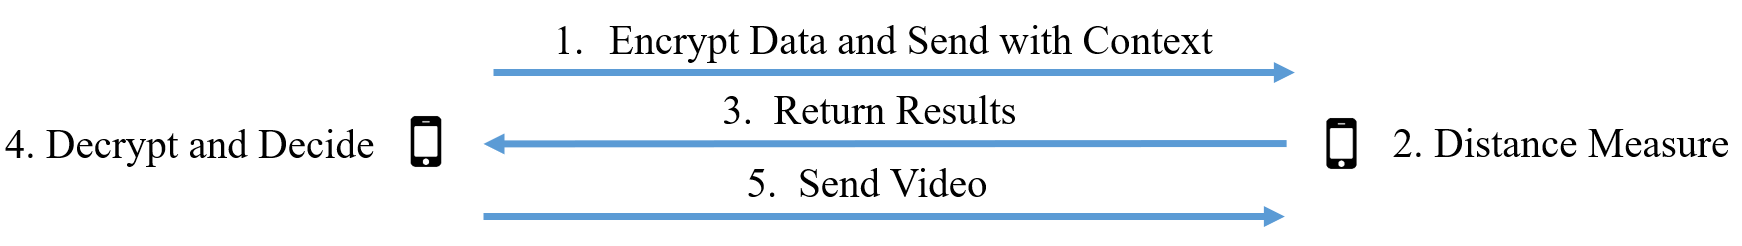
\includegraphics[width=\textwidth]{4 Design/4.3 Peer-to-Peer.png}
    \caption{Peer-to-peer Data Flow}
    \label{fig:peer-to-peer-data-flow}
\end{figure}

To facilitate a peer-to-peer exchange of files shown in Figure \ref{fig:peer-to-peer-data-flow}, GhostPeerShare supports QuickShare \cite{samsung_quick_2020} for Android devices. QuickShare [10] was developed by Samsung as a file-sharing utility application for nearby wireless devices. It leverages Bluetooth to discover nearby wireless devices and optionally uses WiFi to transfer large files between two nodes. QuickShare is accessible through a Flutter plugin that enables users to share data using their device’s native sharing capabilities. This allows each node to asynchronously send and receive files, leveraging a built-in Android feature rather than embedding similar functionality within the Flutter application.


% ========== Chapter 5

\chapter{Results}

In this section, we compare our implementation to the foundational contributions of SSO and Pop-Share. In order to evaluate the accuracy of Fully Homomorphic Encryption Library plugin in Dart, we measure the amount of noise generated during encrypted operations. Next, we compare our implementation of our distance measures using the original pre-processed video frames from SSO. Next, we compare the same video from various angles and determine the accuracy of our implementation. Next, we compare the distance measures for similar scenes against different scenes. Finally, we compare the performance across multiple linux and android devices.

\section{Noise Accumulation}

When performing fully homomorphic operations, a small amount of noise is introduced that affects the accuracy of the decrypted distance measure. If too much noise is accumulated, the plaintext cannot be recovered. Figure 1a represents the baseline Mean Error from Pop-Share, compared to our implementation in Table 5.1. For KLD, our implementation introduced twice the amount of noise than the original. For Cramer Distance, our implementation introduced half of the amount of noise than the original. For Bhattacharyya Coefficient, our implementation introduced half of the amount of noise than the original.

% \usepackage{amsmath}
% \usepackage{graphicx}
% \usepackage{array}

% TODO: 

\begin{table}[h!]
\centering
\begin{tabular}{|c|c|c|}
\hline
\textbf{Function} & \textbf{Pop-Share} & \textbf{GhostPeerShare} \\
\hline
KLD     & $4 \times 10^{-9}$ & $1.78 \times 10^{-6}$ \\
Cramer  & $8 \times 10^{-4}$ & $6.54 \times 10^{-10}$ \\
BC      & $1.3 \times 10^{-1}$ & $6.34 \times 10^{-10}$ \\
\hline
\end{tabular}
\caption{Comparison of Mean Errors for Different Functions}
\end{table}


foobar
\section{Pop-Share Distance Measure}
\label{sec:Pop-Share Distance Measure}
One of the core components of this work is the derivation of Distance Measures; however, the baseline for this implementation was established in Python from SciPy \cite{2020SciPy-NMeth}, sklearn entropy, functions to compute Kullback-Leibler Divergence (KLD) and Cramer’s Distance (CD) for their probability distribution arrays. To ensure a fair comparison between this work and the SSO, the original data is utilized, comparing video frame byte count arrays against network traffic data obtained from Pcap packet byte count arrays. Using this data, the standard deviations of our Dart implementations of KLD and CD are derived and compared to those of the Python implementation.

\begin{figure}[t]
    \centering
    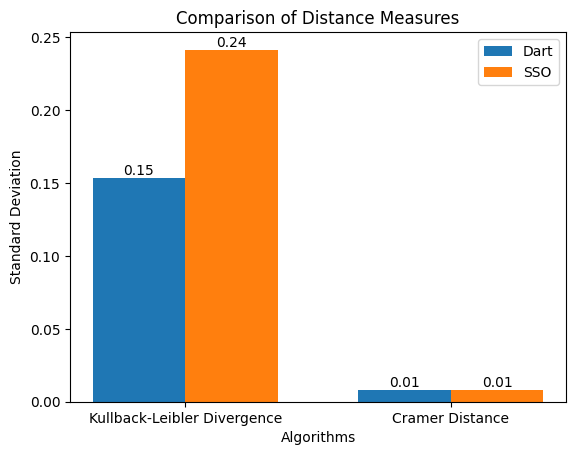
\includegraphics[width=0.8\textwidth]{5 Results/Figures/5.2 Bar Chart.png}
    \caption{Pop-Share Distance Measure}
    \label{fig:pop-share-distance-measure}
\end{figure}

As shown in Figure \ref{fig:pop-share-distance-measure}, our Dart implementation of Kullback-Leibler Divergence (KLD) demonstrates a standard deviation of 0.15, which is lower than the Python implementation’s standard deviation of 0.24. Both implementations incorporate a small epsilon value of $1.0e-12$ to address cases where either $p$ or $q$ are zero. The minimal variance of 0.09 in the Dart implementation suggests that our implementation exhibits less fluctuation compared to the Python implementation, indicating greater stability and consistency in its distance-measure calculations.

For Cramer's Distance (CD), the standard deviation was the same for both implementations at 0.1. This finding aligns with our hypothesis that we should observe the same or very small amounts of variance between the two implementations, further supporting the reliability of the Dart implementation in maintaining consistency across distance measure calculations.

\section{Field of View}
\label{sec:Field of View}

% Better definition of Field of View

A significant contribution from Pop-Share \cite{Lagesse2021-PopShare} was the ability to accurately classify videos from various angles for similarity. Applying the methodology from Similarity of Simultaneous Observation (SSO) \cite{Wu2019-SSO} to compare videos, Pop-Share re-used the pre-processing procedure to convert videos into a byte-count array. Instead of comparing videos to capture network traffic, the application of SSO was altered to compare two videos to each other for similarity. In addition, Pop-Share expanded upon the distance measure implementation to support Fully Homomorphic Encryption, requiring a new set of algorithms that were simplified into basic arithmetic. 

% Training setup

The field-of-view experiment demonstrated that comparing two videos taken at the same time and place of the same subject could be accurately classified using an Artificial Neural Network (ANN). This machine-learning model was trained on the distance measure scores between two videos computing using three probability distribution functions: Kullback-Leibler Divergence (KLD), Bhattacharyya Coefficient (BC), and Cramer Distance (CD). For supervised training, the binary labeling system assigns a one when two scenes are identical, or the first comparison pair is labeled as one to train the model to match similar videos. Otherwise, a zero is assigned for all other comparison pairs, regardless of visual similarity.

Once the videos are aligned and pre-processed, we compute the distance measures of the byte-count arrays representing a one-second segment of each video. In the generated CSV file, each row contains the binary label, followed by all of the scores: KLD, BC, and CD. Since KLD is asymmetric, the scores will differ when comparing A to B versus B to A. We performed an exhaustive comparison of every video, as well as the inverse comparison, to account for asymmetric differences.

\begin{table}[b!]
\centering
\begin{tabular}{lccccc}
\hline
\textbf{System} & \textbf{F1 (\%)} & \textbf{Precision (\%)} & \textbf{Recall (\%)} & \textbf{Accuracy (\%)} & \textbf{Error (\%)} \\
\hline
PoP-Share[2]   & 96.63 & 97.73 & 95.56 & 95.16 & 4.84 \\
Handheld[2]    & 97.97 & 99.32 & 96.67 & 98.00 & 2.00 \\
SSO[6]         & 96.13 & 92.56 & 100.00 & 96.30 & 3.70 \\
GhostPeerShare & 97.09 & 96.14 & 98.05 & 98.05 & 1.95 \\
\hline
\end{tabular}
\caption{Direct Comparison of SSO-based Systems}
\label{table:ann_system_compare}
\end{table}


The Multi-Layer Perceptron (MLP) classifier is part of the scikit-learn \cite{scikit-learn} library. The MLP Classifier used the Limited-memory Broyden-Fletcher-Goldfarb-Shanno (lbfgs) solver to apply weights within the neural network. The model was trained with two hidden layers, each with 10 neurons, and used Rectified Linear Unit (relu), a popular activation function in deep learning. This is the same machine learning model used in SSO and Pop-Share. SSO and Pop-Share were trained for 15 hours using a Nexus 6p and a D-Link Wi-Fi camera (DCS-936L) fixed-motion cameras. The video data from the two cameras include video captures at different resolutions and different relative angles, such as 0, 90, and 180 degrees offset from each other. The videos were also taken at varying distances from each other, ranging from 1 to 25 meters away. In addition, the videos were taken from both an indoor and an outdoor environment with varying levels of motion and lighting conditions.

The Handheld model shown in Table \ref{table:ann_system_compare} was tested using 150 minutes of training data recorded with a Google Pixel 2, a Motorola Moto Z, a Lenovo Phab2 Pro, an LG Nexus 5, and a Huawei Nexus 6p. All phones captured video using h.264 with 3840x2160 resolution at 30 FPS with Optical Image Stabilization (OIS) enabled except the Nexus 5 and Phab2 Pro, which only support 1920x1080 resolution, and the Nexus 6p, which only has Electronic Image Stabilization (EIS). 

GhostPeerShare was trained and tested on a less diverse dataset of 100 minutes of raw videos, which included three twenty-minute videos of low movement featuring an individual sitting at his desk, denoted as \textit{office}, and two twenty-minute videos of high movement capturing an individual vacuuming his living room, denoted as \textit{vaccum} in Appendix Table \ref{table:appendix_ann}. The video data was recorded on fixed-motion phones: Pixel 3XL using h.264 with 1920x1080 resolution at 30 FPS and Samsung S9 using h.264 with 1280x720 resolution at 30 FPS. The phones were placed at different relative angles and varying distances. However, all videos were filmed indoors with relatively similar lighting. 

For a practical analysis, the ANN was trained on a high-movement scene and tested on a low-movement scene, achieving an Accuracy and Recall score of 98.05\%, a Precision Score of 96.14\%, and an F1 Score of 97.09\%. The lack of diversity within the training and testing dataset is likely a contributing factor to the lower scores for F1 and Precision. Recording more video data in various locations with a wide variety of devices and environments, the F1 and Precision scores may improve. This model demonstrates that GhostPeerShare consistently generates a unique representation of video data and can accurately predict the binary label given the three distance measure scores for a different dataset.

\section{Scene Distance Measure}
\label{sec:Scene Distance Measure}

The purpose of this experiment is to investigate the range of distance measure scores from our training data in Section \ref{sec:Field of View}. Figure \ref{fig:scene-distance-measure} illustrates the average distance measure score for each algorithm from our dataset, comparing different and same scenes. The scenes were labeled according to our binary labeling system, where one indicates similar scenes and zero otherwise. The graph also includes the standard error above and below the mean distance measure, indicating the range within which the true mean distance measure score is expected. This graph mirrors the same experiment performed by Pop-Share. Pop-Share's training data was much more diverse, with around 16 hours of raw video spanning across various environments and recorded from many devices. GhostPeerShare was training on a total of 100 minutes of indoor video data recorded by two phones.

\begin{figure}[t]
    \centering
    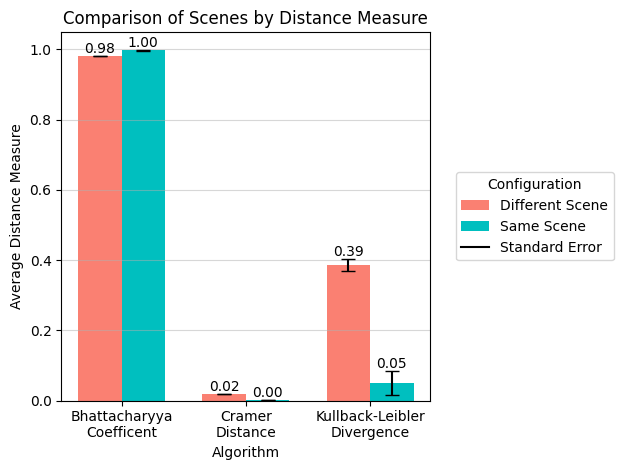
\includegraphics[width=0.8\textwidth]{5 Results/Figures/5.4 Bar Chart.png}
    \caption{Scene Distance Measure}
    \label{fig:scene-distance-measure}
\end{figure}

For the Bhattacharyya Coefficient, a perfect score of 1.00 indicates that the two scenes are identical, while a score of zero denotes no overlap. From Pop-Share, the same pattern was found for the Bhattacharyya Coefficient, containing little variance between different and same scenes and significantly less standard error than other metrics. In our experiments, we observed a 0.02 variance between the distance measures for different and same scenes. This minimal variance is likely attributed to the uniformity of the scene types recorded, as both sets were filmed indoors, and the fact that the same devices were used during the experiments, which limited the diversity in the captured footage.

For Cramer Distance, a perfect score of 0.00 indicates that the two scenes are identical, while a score of 1.0 is the maximum distance between two probability distributions. From Pop-Share, Cramer Distance contained a significant absolute difference of around 0.25 between different and same scenes. In our experiments, we observed significantly less variance, 0.02, between the distance measures for different and same scenes. The lack of variance is likely attributed to the limited data used in our experiments compared to Pop-Share. 

For the Kullback-Leibler Divergence (KLD), a perfect score of 0.00 indicates that two scenes are identical, while the upper limit is infinity; the smaller the score, the more similar the two probability distributions are. From Pop-Share, KLD was the leading indicator of dissimilarity, however, their experiments contained significant variance greater than 1 between different and same scenes. In our experiments, we observed a 0.34 variance between the distance measures for different and same scenes. This represents the highest variance observed among all of our distance measures and serves as a significant indicator that two scenes may be different.

The key takeaway from our experiments is that while the individual scores for the distance measures exhibit minimal variance, they still effectively differentiate between similar and different scenes. This consistency suggests that the implemented algorithms can reliably assess similarity, even in scenarios where the overall variation in scores is low. Consequently, the results highlight the robustness of our methodology in accurately identifying scene differences, which is crucial for applications requiring precise content analysis without revealing the underlying video data.

\section{Performance}

To compare this implementation to the mobile Proof of Presence Share (Pop-Share) application, preprocessing speed for one-minute videos was benchmarked, and the duration of encrypted operations was measured against plaintext operations. This comparison allowed for assessment of the implementation's efficiency and quantification of the impact of encryption on performance.

\begin{table}[b!]
\centering
\begin{tabular}{|l|c|c|c|}
\hline
\textbf{System} & \textbf{Average (s)} & \textbf{Min (s)} & \textbf{Max (s)} \\
\hline
PC              & 111.25 & 13.00 & 321.00 \\
Samsung S9      & 421.62 & 180.00 & 755.50 \\
Pixel 3XL       & 454.50 & 171.00 & 875.00 \\
\hline
\end{tabular}
\caption{Pre-processing duration (in seconds) for a one minute video.}
\label{table:preprocessing_times}
\end{table}
 

Experiments used one-minute videos with h264 encoding, results shown in Table \ref{table:preprocessing_times}. On a Pixel 3 XL mobile phone, preprocessing with OpenCV required 438 seconds (about 7.3 minutes) on average. In contrast, Pop-Share on a Pixel 2 took only 17 seconds on average using FFMpeg. This difference stems from the use of different libraries for preprocessing. Limited operating system support for FFMpeg plugins restricted plugin selection to one compatible with both Linux and Android. On a Linux PC with OpenCV, preprocessing  took 111 seconds (about 2 minutes) on average. This result demonstrates the PC operated approximately four times faster than the average of the two mobile devices. The disparity likely arises from differences in CPU thread availability and speed. The PC has 32 threads at 3.4 GHz, while both Android phones have 8 threads at about 2.5 GHz.

Dart code executes in isolates, which resemble threads but with separate memory allocations. Flutter applications perform all operations on a single isolate. Although the implementation creates an isolate to count bytes in each one-second segment, it does not incorporate parallelism. The frame parsing process remains sequential. This design choice prioritized stability over performance to ensure consistent operation. Table \ref{table:preprocessing_times} presents the execution times on mobile and Linux desktop environments. The data reveals substantial differences that highlight inefficiencies in the mobile implementation. These inefficiencies prevent achievement of operational targets relative to the Pop-Share baseline. Potential optimization strategies are explored in Section DISCUSSION.

For encryption and encoding of each distance measure varies, as the parameters to the Fully Homomorphic distance measure implementation is different, described in further detail in Section METHODS. Unfortunately, we cannot compare these metrics to Pop-Share as they were not explicitly mentioned in their evaluation. However, our approach treats the preprocessing of video frames as an independent transaction, separate from the encoding and encryption steps. Shown in Table \ref{table:cryptography}, the Kullback-Leibler Divergence (KLD) encryption is about twice that of Bhattacharyya and Cramer due to the requirement of double the amount of data. This pattern was also indicated in Pop-Share.

\begin{table}[t]
\caption{Comparison of Cryptography (in Milliseconds) on Android}
\centering
\begin{tabular}{|l|c|c|c|}
\hline
\textbf{Algorithm} & \textbf{Encryption (ms)} & \textbf{Decryption (ms)} \\
\hline
KLD & 1019.00 & 229.88 \\
BC  & 503.00 & 140.25 \\
CD  & 507.12 & 217.50 \\
\hline
\end{tabular}
\label{table:cryptography}
\end{table}


The Fully Homomorphic Encryption computations, shown in Table \ref{table:fhe_operations}, are within ±20\% of Pop-Share, validating our abstraction design and interface implementation. This performance increase is likely due to the advancements in Microsoft SEAL, Pop-Share used version v3.3, while our implementation uses v4.1.

\begin{itemize}
    \item Kullback-Leibler Divergence: Pop-Share reported an average time of 400 milliseconds, whereas our implementation achieved 346 milliseconds, representing a 13.5\% increase in performance.
    \item Cramer Distance: Pop-Share reported an average time of 386 milliseconds, whereas our implementation achieved 310 milliseconds, representing a 19.4\% increase in performance.
    \item Bhattacharyya Coefficient: Pop-Share reported an average time of 186 milliseconds, whereas our implementation yielded 203 milliseconds, representing a 9.1\% decrease in performance.
\end{itemize}

\begin{table}[t]
\caption{Comparison of FHE Operations (in Milliseconds) on Android}
\centering
\begin{tabular}{|l|c|c|c|}
\hline
\textbf{Algorithm} & \textbf{FHE Compute (ms)} & \textbf{Plaintext Compute (ms)} \\
\hline
KLD & 345.38 & 1.12 \\
BC  & 202.38 & 0.41 \\
CD  & 309.38 & 0.45 \\
\hline
\end{tabular}
\label{table:fhe_operations}
\end{table}


The plaintext computations, shown in Table \ref{table:fhe_operations}, are much faster than expected, a significant performance increase in Dart compared to Python implementation. This performance increase may be due to the underlying data structure selection in Dart.

\begin{itemize}
    \item Kullback-Leibler Divergence: Pop-Share reported an average time of 3.8 milliseconds, whereas our implementation achieved 1.12 milliseconds, representing a 70.5\% increase in performance.
    \item Cramer Distance: Pop-Share reported an average time of 5.2 milliseconds, whereas our implementation achieved 0.45 milliseconds, representing a 91.35\% increase in performance.
    \item Bhattacharyya Coefficient: Pop-Share reported an average time of 3.2 milliseconds, whereas our implementation achieved 0.41 milliseconds, representing a 87.5\% increase in performance.
\end{itemize}

To extract a distance measure from the archive, we calculate the score by decrypting each ciphertext in the modified byte count array and summing all the elements. Cramer's method differs as it involves calculating the square root of the result. Shown in Table \ref{table:cryptography}, Pop-Share had an average duration of 250 milliseconds, while our Android implementation took 588 milliseconds. Although the difference is insignificant, it suggests potential differences in our implementation.

In total on Android, to upload and convert the video frames into byte count arrays took, on average, 438 seconds (7 minutes) for a one-minute video. To encode, encrypt, and generate the archive took, on average, 2 seconds. When performing Fully Homomorphic Encryption (FHE) operations on all ciphertexts took, on average, 857 milliseconds. Finally, decryption took, on average, 588 milliseconds. In total, it took 3.4 seconds to derive a similarity score using FHE. As the preprocessing is expensive, it only has to be performed once for every video uploaded to the application.

Overall, this study benchmarked the performance of our implementation on Android to the existing Pop-Share application. The results showed significantly slower preprocessing times due to library limitations, but the encryption, computation, and decryption times were competitive to Pop-Share. Our implementation demonstrates high efficiency of the Fully Homomorphic Encryption operations. Notably, plaintext computations were significantly faster in our implementation.


% ========== Chapter 6

\chapter{Discussion}

This chapter examines the implementation and future potential of the Fully Homomorphic Encryption Library (FHEL) Plugin and the Distance Measure Plugin. The FHEL Plugin enhances access to Fully Homomorphic Encryption (FHE) for mobile and Linux applications by integrating Microsoft SEAL, allowing Dart and Flutter developers to improve privacy in their apps with clear documentation and user-friendly interfaces. The Distance Measure Plugin further adds value by implementing advanced statistical measures like Kullback-Leibler Divergence, Cramer Distance, and Bhattacharyya Coefficient, facilitating computations on encrypted data. Together, these plugins support efficient resource management and high performance, establishing a foundation for future innovations in secure data exchange and privacy in mobile applications.

\section{Qualitative Analysis}
The modular implementation of the Fully Homomorphic Encryption Library (FHEL) Plugin represents a significant advancement in Microsoft SEAL, increasing the availability of Fully Homomorphic Encryption (FHE) to the mobile community and Linux applications. This plugin integrates Microsoft SEAL, enabling Dart and Flutter developers to leverage advanced cryptographic capabilities, thereby enhancing privacy in mobile applications. The well-structured documentation and user interfaces ensure that developers can navigate the complexities of the tool with ease. Early feedback indicates that the plugin is user-friendly and effective, although there remains potential for further refinements, particularly in supporting additional backend libraries.
The Distance Measure Plugin complements the FHEL Plugin by providing implementations of state-of-the-art statistical measures, Kullback-Leibler Divergence, Cramer Distance, and Bhattacharyya Coefficient, as well as their fully homomorphic encryption counterpart to perform computations directly on encrypted data.
This modular architecture facilitates efficient resource management and high performance while allowing for the seamless integration of future cryptographic algorithms. Together, these developments will advance the field of secure data analysis and establish a solid foundation for future innovations, reinforcing the importance of privacy in contemporary applications.

\section{Limitations}
The implementation of the Fully Homomorphic Encryption Library (FHEL) Plugin, the Distance Measure Plugin, and the Flutter application faces several limitations that may impact their usability and performance.
A notable limitation is the availability of FFmpeg, which is only supported on Android and iOS. This restriction obstructs our ability to use a consistent video preprocessing library and methods, hindering the direct re-implementation of the approach from Pop-Share. Additionally, while OpenCV has been utilized for certain features, its performance and compatibility may vary across different operating systems, potentially leading to inconsistencies in the application's behavior.
While the plugins incorporate multi-threaded operations to enhance performance, executing these operations on mobile devices may not be optimal. Pre-processing tasks could suffer from the constraints of mobile hardware, resulting in slower performance or increased latency during computations. This limitation can particularly affect real-time processing capabilities when handling large datasets or multiple video streams.
These limitations underscore the need for continuous development and optimization to ensure consistent performance and broader compatibility across various platforms and use cases.

\section{Future Work}
Expanding the range of statistical measures in the Distance Measure Plugin will allow for a more comprehensive analysis of data similarity, with plans to integrate additional metrics such as Dynamic Time Warping and Jensen-Shannon Divergence.
There is also a clear path toward refining the GhostPeerShare application for production use, involving rigorous testing and performance optimization. Currently focused on Android and Linux, future efforts will target cross-platform support for iOS, macOS, and Windows, broadening accessibility for users. Additionally, enhanced user support and documentation will be developed to assist developers in effectively utilizing the plugins, while ongoing performance optimization will address mobile environment challenges, such as refining multi-threading capabilities and improving memory management. Lastly, actively soliciting and incorporating user feedback will ensure the plugins evolve to meet the needs of their user base, reinforcing their significance in secure data computations and paving the way for future innovations in Fully Homomorphic Encryption within the Flutter and Dart communities.


% ========== Chapter 7

\chapter{Conclusion}
This work demonstrates the feasibility and effectiveness of integrating Fully Homomorphic Encryption into mobile applications using our Fully Homomorphic Encryption Library plugin, written in Dart. By leveraging Microsoft SEAL, our implementation enables high-performance encrypted computations on mobile devices, meeting critical privacy and security demands without compromising user experience.

Through our Distance Measure plugin, we achieved consistent and accurate similarity detection scores between videos using Kullback-Leibler Divergence (KLD), Bhattacharyya Coefficient, and Cramer’s Distance. Our results reveal that both Cramer Distance and Bhattacharyya Coefficient exhibit lower noise accumulation compared to KLD, underscoring the importance of distance measure selection based on computational requirements and noise sensitivity. The reduced variance in our Dart implementation compared to the Python baseline further highlights its stability and reliability for mobile applications. The advancements within SEAL v4.1 have contributed significantly to our system’s performance. However, the pre-processing library, OpenCV, has negatively impacted the performance of video processing and feature extraction compared to FFmpeg.

Ultimately, this project lays the foundation for future applications of FHE in mobile environments, especially in fields like healthcare and secure data exchange, where privacy and accuracy are paramount. By making SEAL accessible within a mobile-compatible, modular framework, we are opening pathways for broader adoption of FHE and setting the stage for innovation in mobile security.


%
% ==========   Bibliography
%
\nocite{*}   % include everything in the uwthesis.bib file
\bibliographystyle{ieeetr}
\bibliography{uwthesis}
%
% ==========   Appendices
%
\appendix
\raggedbottom\sloppy
 
% ========== Appendix A
 
\chapter{Tables}
 
\begin{table}[h!]
\centering
\begin{tabular}{lcccc}
\hline
\textbf{Configuration} & \textbf{Accuracy (\%)} & \textbf{Precision (\%)} & \textbf{Recall (\%)} & \textbf{F1-Score (\%)} \\
\hline
office\_default                   & 97.42 & 94.90 & 97.42 & 96.14 \\
office\_gridSearch                & 99.85 & 99.85 & 99.85 & 99.85 \\
vacuum\_default                   & 97.58 & 95.21 & 97.58 & 96.38 \\
vacuum\_gridSearch                & 99.65 & 99.66 & 99.65 & 99.64 \\
office\_vs\_vacuum\_default       & 99.82 & 100.00 & 99.82 & 99.91 \\
office\_vs\_vacuum\_gridSearch    & 99.95 & 100.00 & 99.95 & 99.98 \\
train\_office\_test\_vacuum\_default  & 97.23 & 94.54 & 97.23 & 95.86 \\
train\_vacuum\_test\_office\_default  & 98.05 & 96.14 & 98.05 & 97.09 \\
\hline
\end{tabular}
\caption{Performance metrics for different configurations.}
\label{table:appendix_ann}
\end{table}


\end{document}
